%%%%%%%%%%%%%%%%%%%%%%%%%%%%%%%%%%%%%%%%%%%%%%%%%%%%%%%%%%%%%%%%%%%%%%%%%%%%%%%%
\section{Análisis comparativo de estrategias}
\label{sec:exp_comparativo}
%%%%%%%%%%%%%%%%%%%%%%%%%%%%%%%%%%%%%%%%%%%%%%%%%%%%%%%%%%%%%%%%%%%%%%%%%%%%%%%%

En esta sección se presenta una comparación directa de las tres estrategias propuestas —Frontera, Ruta Planificada y Predictiva— entre sí y frente a la línea de base Greedy, sobre las mismas 10 configuraciones (entorno $\times$ número de actores). El análisis se organiza en tres bloques: resultados desagregados por métrica, puntuación compuesta global y análisis de trade-offs con recomendaciones de uso.

\subsection{Resultados comparativos por métrica}
\label{sec:exp_comp_metricas}

Las Tablas~\ref{tab:comp_ghost},~\ref{tab:comp_entropy} y~\ref{tab:comp_frames} presentan los valores finales de cada métrica para las cuatro estrategias. En cada fila se resalta en negrita el mejor valor por configuración. Para celdas fantasma el mejor valor es el menor; para entropía y frames, el mayor.

\begin{table}[htbp]
    \centering
    \caption{Celdas fantasma (valor final, menor es mejor) por configuración y estrategia. En negrita, el mejor valor de cada fila.}
    \label{tab:comp_ghost}
    \begin{tabular}{lrrrr}
        \toprule
        \textbf{Configuración} & \textbf{Frontera} & \textbf{Ruta Plan.} & \textbf{Predictiva} & \textbf{Greedy} \\
        \midrule
        house-0   & 16  & 20  & 30  & \textbf{15}  \\
        office-0  & 21  & 34  & 14  & \textbf{13}  \\
        house-5   & 53  & 59  & \textbf{0}   & 81  \\
        office-5  & 92  & \textbf{68}  & 99  & 78  \\
        house-10  & \textbf{0}   & 130 & \textbf{0}   & 83  \\
        office-10 & 105 & 27  & \textbf{18}  & 125 \\
        house-15  & 155 & 216 & \textbf{0}   & 118 \\
        office-15 & \textbf{24}  & 220 & \textbf{0}   & 153 \\
        house-20  & \textbf{0}   & 72  & \textbf{0}   & 131 \\
        office-20 & \textbf{0}   & 51  & 63  & 83  \\
        \bottomrule
    \end{tabular}
\end{table}

En la Tabla~\ref{tab:comp_ghost} se observa que la estrategia Predictiva obtiene el mejor resultado en \textbf{7 de las 10} configuraciones en celdas fantasma, logrando cero ghost cells en cinco de ellas. La estrategia Frontera comparte el mejor resultado en house-10 y house-20, y es la única que alcanza cero en office-20. La estrategia Ruta Planificada solo predomina en office-5, y presenta los peores resultados de las tres estrategias propuestas en house-10, house-15 y office-15, donde supera incluso a Greedy en número de ghost cells. Las configuraciones de 0 actores son las únicas en que Greedy registra el menor número de celdas fantasma, lo que es coherente con la ausencia de obstáculos dinámicos que penalicen a las tres estrategias propuestas.

\begin{table}[htbp]
    \centering
    \caption{Entropía del mapa (valor final $\times 10^{-4}$, mayor es mejor) por configuración y estrategia. En negrita, el mejor valor de cada fila.}
    \label{tab:comp_entropy}
    \begin{tabular}{lrrrr}
        \toprule
        \textbf{Configuración} & \textbf{Frontera} & \textbf{Ruta Plan.} & \textbf{Predictiva} & \textbf{Greedy} \\
        \midrule
        house-0   & 1{,}43 & \textbf{1{,}83} & 0{,}10 & 1{,}29 \\
        office-0  & 1{,}33 & 1{,}21 & 1{,}10 & \textbf{2{,}06} \\
        house-5   & 0{,}95 & 0{,}55 & 1{,}10 & \textbf{1{,}67} \\
        office-5  & 0{,}78 & 1{,}01 & 0{,}85 & \textbf{1{,}07} \\
        house-10  & \textbf{1{,}51} & 1{,}34 & 0{,}62 & 0{,}66 \\
        office-10 & \textbf{1{,}49} & 0{,}78 & 1{,}40 & 1{,}27 \\
        house-15  & \textbf{1{,}24} & 1{,}22 & 0{,}76 & 0{,}09 \\
        office-15 & 1{,}12 & \textbf{1{,}19} & 0{,}12 & 0{,}89 \\
        house-20  & 0{,}48 & 1{,}11 & 0{,}10 & \textbf{1{,}88} \\
        office-20 & 0{,}12 & 0{,}15 & 0{,}54 & \textbf{1{,}21} \\
        \bottomrule
    \end{tabular}
\end{table}

La Tabla~\ref{tab:comp_entropy} revela que la estrategia Frontera es la que más frecuentemente maximiza la entropía del mapa, ganando en \textbf{5 de las 10} configuraciones, seguida de Ruta Planificada con 4 y Predictiva con solo 2. Greedy domina en las configuraciones con 0 actores (ambos entornos) y con alta densidad (house-20 y office-20). Este patrón indica que la estrategia Predictiva, al priorizar rutas con menor interferencia dinámica, tiende a concentrar la exploración en zonas ya conocidas, sacrificando la diversidad del mapa. La estrategia Frontera, con su evaluación simple del punto de destino, produce un patrón de exploración más diversificado.

\begin{table}[htbp]
    \centering
    \caption{Frames totales procesados (valor final acumulado, mayor es mejor) por configuración y estrategia. En negrita, el mejor valor de cada fila.}
    \label{tab:comp_frames}
    \begin{tabular}{lrrrr}
        \toprule
        \textbf{Configuración} & \textbf{Frontera} & \textbf{Ruta Plan.} & \textbf{Predictiva} & \textbf{Greedy} \\
        \midrule
        house-0   & 364 & 481 & \textbf{620} & 217 \\
        office-0  & 478 & 534 & \textbf{613} & 555 \\
        house-5   & 439 & 471 & 449 & \textbf{577} \\
        office-5  & 444 & 519 & 523 & \textbf{648} \\
        house-10  & 390 & 401 & 419 & \textbf{454} \\
        office-10 & 400 & 499 & \textbf{638} & 601 \\
        house-15  & 356 & 339 & 340 & \textbf{597} \\
        office-15 & 366 & 377 & 509 & \textbf{607} \\
        house-20  & 353 & \textbf{477} & 437 & 265 \\
        office-20 & 379 & 570 & \textbf{596} & 98  \\
        \bottomrule
    \end{tabular}
\end{table}

En la Tabla~\ref{tab:comp_frames} se observa que la estrategia Predictiva procesa más frames en \textbf{5 de las 10} configuraciones, siendo la de mayor throughput en 0 actores (ambos entornos) y en office-10 y office-20. Greedy domina en densidades de 5 y 15 actores, donde las estrategias propuestas penalizan la selección de fronteras y reducen la frecuencia de desplazamiento. Las tres estrategias propuestas superan ampliamente a Greedy en las configuraciones de 20 actores, donde Greedy sufre interrupciones frecuentes por congestión.

\subsection{Puntuación compuesta}
\label{sec:exp_comp_score}

La Figura~\ref{fig:comp_score_config} presenta la puntuación compuesta de las cuatro estrategias en cada configuración, calculada con los pesos establecidos en la Sección~\ref{sec:exp_calibracion}: 40\% celdas fantasma, 35\% entropía del mapa y 25\% frames procesados, sobre normalización global min-máx aplicada a la unión de los valores de las cuatro estrategias.

\begin{figure}[htbp]
    \centering
    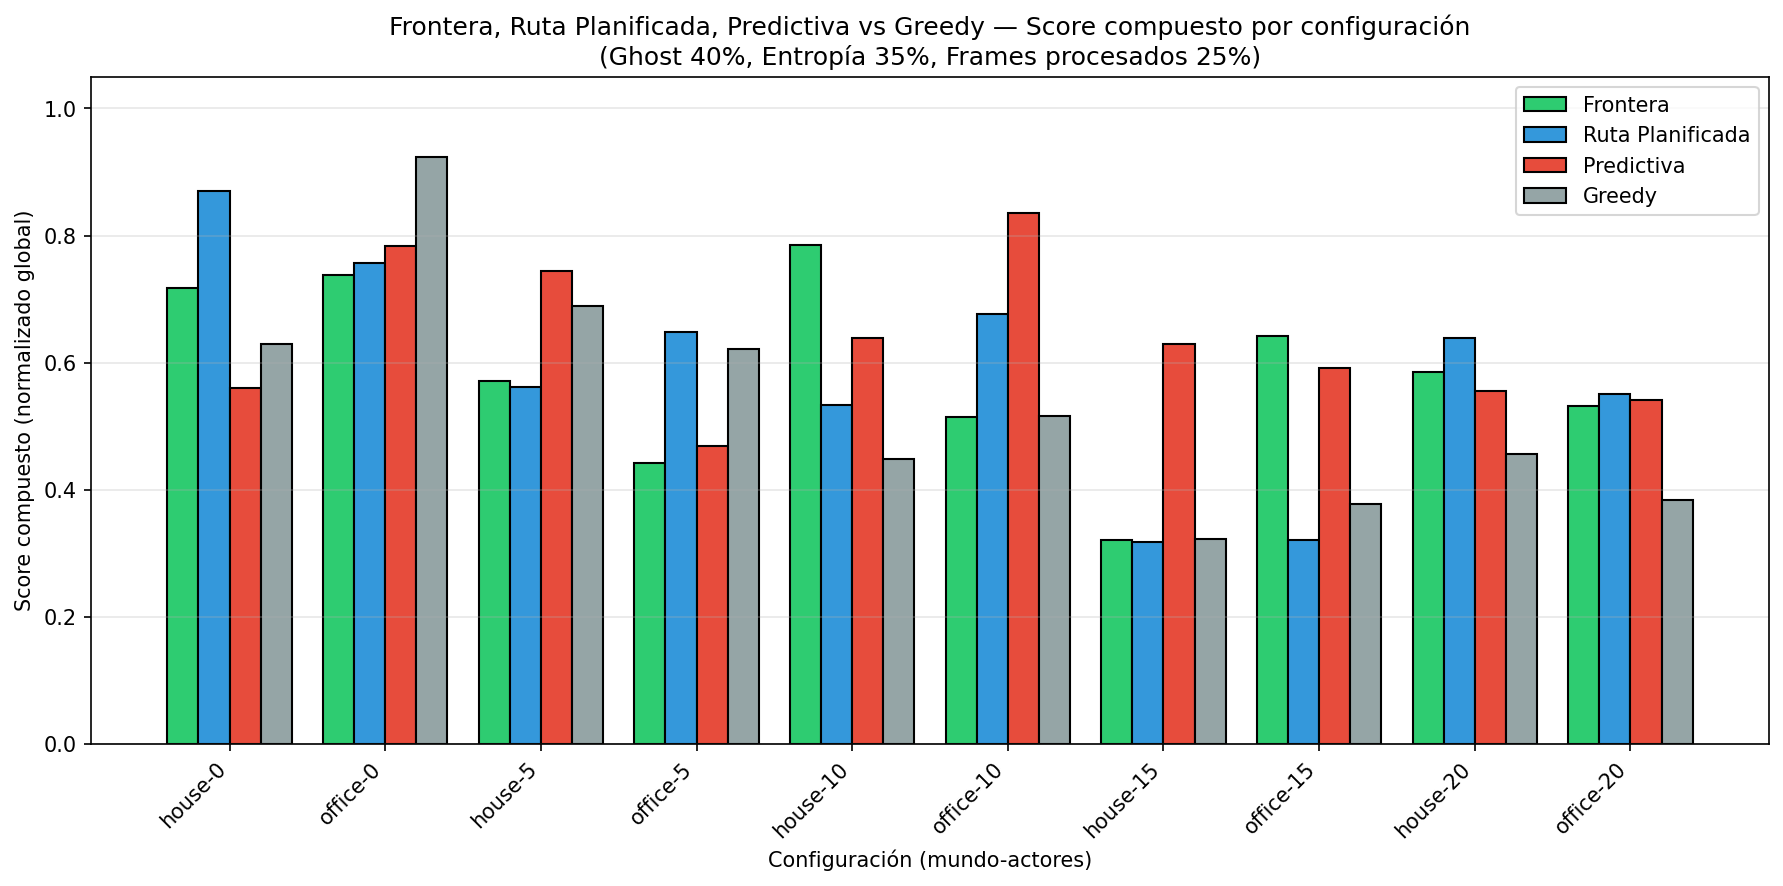
\includegraphics[width=\textwidth]{figures/experiments/comparativo/validation_comparison_01_score_por_config.png}
    \caption{Puntuación compuesta de las cuatro estrategias por configuración. Se muestra en qué configuraciones cada estrategia propuesta supera a Greedy.}
    \label{fig:comp_score_config}
\end{figure}

\begin{figure}[htbp]
    \centering
    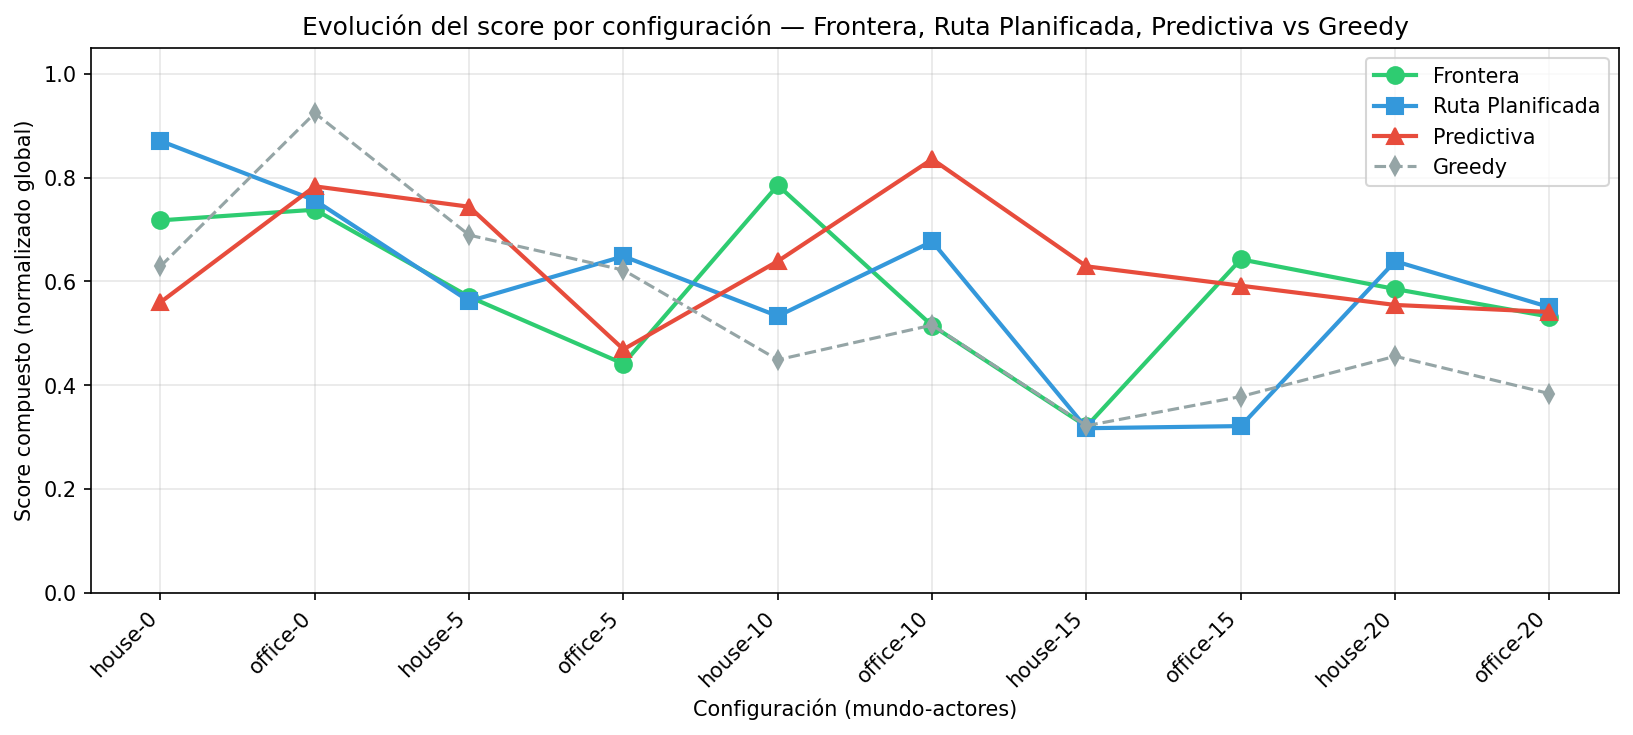
\includegraphics[width=\textwidth]{figures/experiments/comparativo/validation_comparison_04_lineas_score.png}
    \caption{Evolución de la puntuación compuesta por configuración (representación en líneas). Permite identificar el comportamiento relativo de las estrategias a lo largo del gradiente de densidad de actores.}
    \label{fig:comp_score_lineas}
\end{figure}

En las Figuras~\ref{fig:comp_score_config} y~\ref{fig:comp_score_lineas} se aprecia que la estrategia Predictiva obtiene la puntuación compuesta más alta en \textbf{7 de las 10} configuraciones frente a Greedy, mientras que Frontera y Ruta Planificada ganan en \textbf{5 de las 10} cada una. Las Figuras~\ref{fig:comp_victorias_estrategia} y~\ref{fig:comp_victorias_metrica} resumen este resultado.

\begin{figure}[htbp]
    \centering
    \begin{subfigure}[b]{0.48\textwidth}
        \centering
        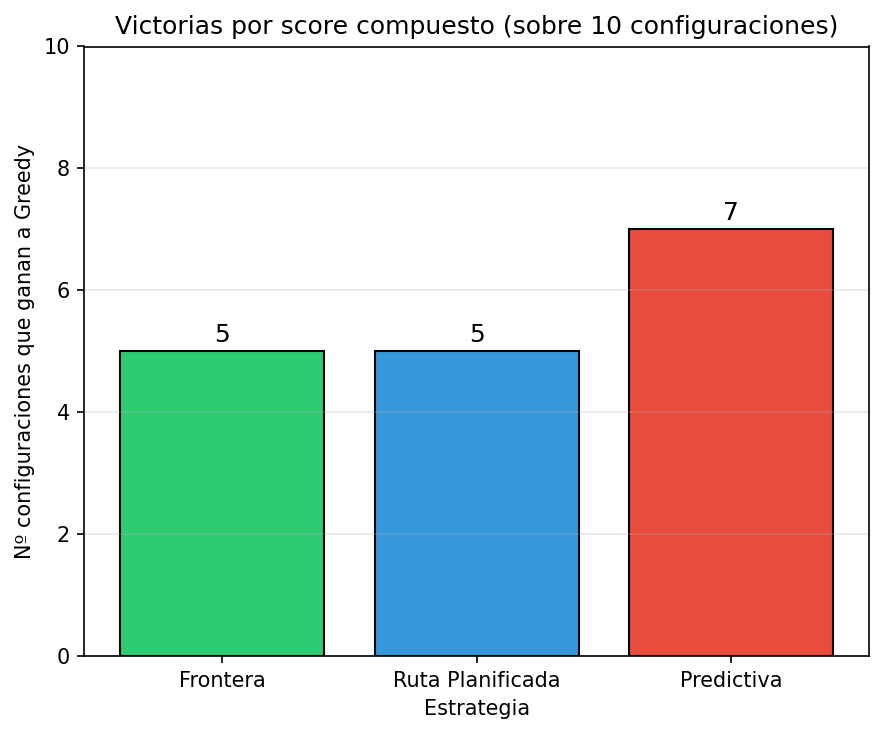
\includegraphics[width=\textwidth]{figures/experiments/comparativo/validation_comparison_02_victorias_por_estrategia.png}
        \caption{Victorias por estrategia (vs Greedy, score compuesto).}
        \label{fig:comp_victorias_estrategia}
    \end{subfigure}
    \hfill
    \begin{subfigure}[b]{0.48\textwidth}
        \centering
        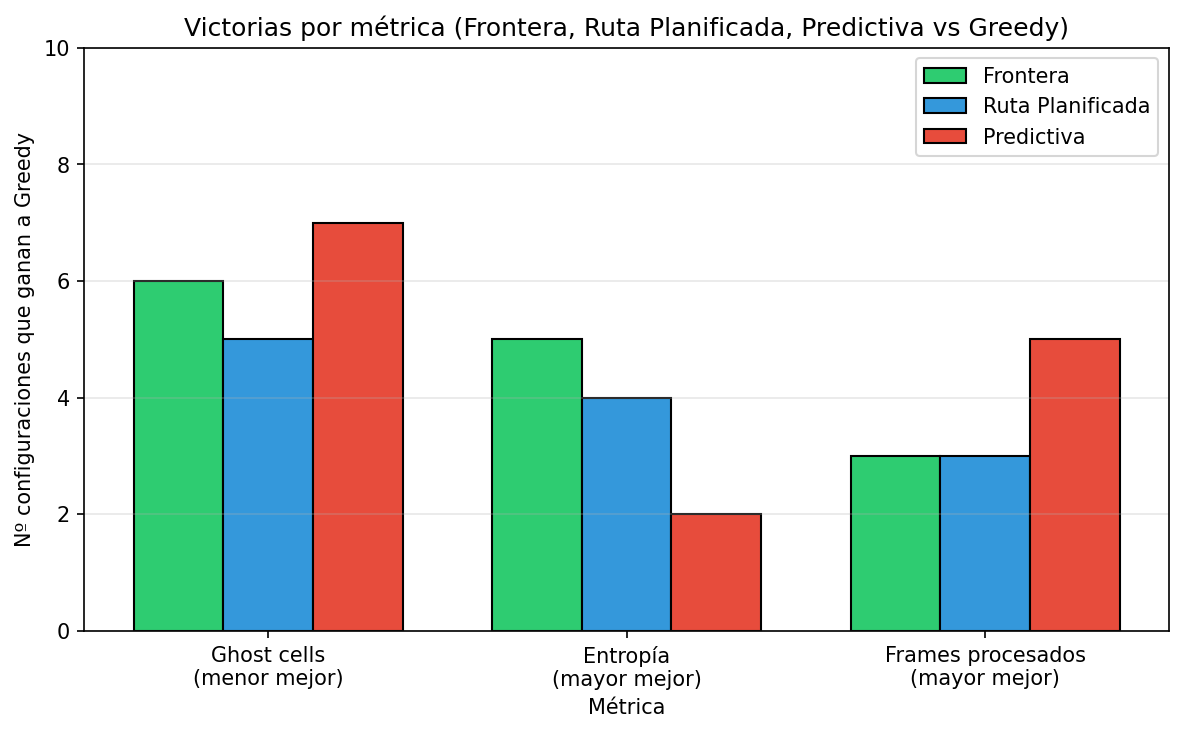
\includegraphics[width=\textwidth]{figures/experiments/comparativo/validation_comparison_03_victorias_por_metrica.png}
        \caption{Victorias por métrica individual (vs Greedy).}
        \label{fig:comp_victorias_metrica}
    \end{subfigure}
    \caption{Recuento de victorias de cada estrategia propuesta frente a Greedy, por score compuesto y por métrica individual.}
    \label{fig:comp_victorias}
\end{figure}

La Figura~\ref{fig:comp_victorias_metrica} pone de manifiesto los perfiles diferenciados de cada estrategia:
\begin{itemize}
    \item \textbf{Predictiva}: máximo rendimiento en celdas fantasma (7/10) y en frames procesados (5/10); rendimiento mínimo en entropía (2/10).
    \item \textbf{Frontera}: perfil más equilibrado; mejor estrategia en entropía (5/10) y segunda en celdas fantasma (6/10).
    \item \textbf{Ruta Planificada}: menor rendimiento en celdas fantasma (5/10) que Frontera, a pesar de su mayor sofisticación en el modelo de costo dinámico; igual rendimiento en frames (3/10) pero mejores magnitudes en los casos que gana.
\end{itemize}

La Tabla~\ref{tab:comp_mejor_por_config} sintetiza, para cada configuración, qué estrategia propuesta obtuvo el mayor score compuesto entre las tres.

\begin{table}[htbp]
    \centering
    \caption{Estrategia con mayor puntuación compuesta entre Frontera, Ruta Planificada y Predictiva, por configuración. Se indica si esa estrategia además supera a Greedy.}
    \label{tab:comp_mejor_por_config}
    \begin{tabular}{lccc}
        \toprule
        \textbf{Configuración} & \textbf{Mejor estrategia} & \textbf{Supera a Greedy} \\
        \midrule
        house-0   & Ruta Planificada & Sí \\
        office-0  & Predictiva       & No \\
        house-5   & Predictiva       & Sí \\
        office-5  & Ruta Planificada & No \\
        house-10  & Frontera         & Sí \\
        office-10 & Predictiva       & Sí \\
        house-15  & Predictiva       & Sí \\
        office-15 & Frontera         & Sí \\
        house-20  & Ruta Planificada & Sí \\
        office-20 & Predictiva       & Sí \\
        \bottomrule
    \end{tabular}
\end{table}

Se observa que ninguna estrategia domina en todas las configuraciones: Predictiva lidera en 5 de 10, Frontera en 2 de 10 y Ruta Planificada en 3 de 10. Las únicas dos configuraciones en que ninguna de las tres estrategias supera a Greedy son office-0 y office-5, ambas con baja densidad de actores en el entorno más grande, donde la exploración sin restricciones dinámicas resulta más eficiente.

\subsection{Trade-offs y recomendaciones de uso}
\label{sec:exp_comp_tradeoffs}

Los resultados permiten identificar tres trade-offs estructurales que caracterizan el comportamiento del sistema:

\textbf{Precisión vs.\ exploración.} La estrategia Predictiva minimiza las celdas fantasma a costa de reducir la entropía del mapa. Al evitar proactivamente las rutas con mayor interferencia dinámica futura, el robot tiende a regresar a zonas ya conocidas, lo que limita la diversidad de observaciones. La estrategia Frontera, con su evaluación más simple, produce un patrón de exploración más amplio aunque con mayor riesgo de acumular ghost cells. Este trade-off sugiere que la elección entre Predictiva y Frontera depende de si la prioridad es la precisión del mapa o su cobertura.

\textbf{Sofisticación del modelo vs.\ rendimiento observado.} La estrategia Ruta Planificada incorpora más información que Frontera —evaluando el trayecto completo— pero obtiene peores resultados en celdas fantasma en 7 de las 10 configuraciones. Esto ilustra que un modelo de costo dinámico más complejo no garantiza mejor rendimiento si no anticipa el estado futuro del entorno. Solo la estrategia Predictiva, que incorpora predicción de trayectorias, logra superar consistentemente a las dos estrategias anteriores en la métrica de mayor peso (celdas fantasma).

\textbf{Densidad de actores.} Las tres estrategias propuestas muestran mayor ventaja sobre Greedy a medida que aumenta la densidad de actores. Con 0 o 5 actores, Greedy es competitivo o superior en la mayoría de configuraciones, especialmente en el entorno office. A partir de 10 actores las estrategias propuestas ganan de forma más consistente, siendo la densidad de 15--20 actores el escenario donde la diferencia es más marcada.

Sobre la base de estos trade-offs, se presenta la Tabla~\ref{tab:comp_recomendaciones} como guía de selección de estrategia según el objetivo del sistema.

\begin{table}[htbp]
    \centering
    \caption{Recomendaciones de selección de estrategia según el objetivo de optimización.}
    \label{tab:comp_recomendaciones}
    \begin{tabular}{lp{7cm}}
        \toprule
        \textbf{Objetivo principal} & \textbf{Estrategia recomendada} \\
        \midrule
        Maximizar precisión del mapa (menos ghost cells) & Predictiva \\
        Maximizar exploración (mayor entropía) & Frontera \\
        Maximizar throughput (más frames procesados) & Predictiva \\
        Balance entre las tres métricas & Frontera \\
        Entorno con $\leq 5$ actores & Greedy o Frontera \\
        Entorno con $\geq 10$ actores & Predictiva \\
        \bottomrule
    \end{tabular}
\end{table}

\subsection{Conclusión del capítulo}
\label{sec:exp_conclusion}

En este capítulo se evaluaron tres estrategias de planificación de próxima vista para el sistema AlfredZ bajo distintas condiciones de densidad de actores dinámicos, comparándolas frente a la línea de base Greedy en los entornos house y office.

Los resultados muestran que la progresión de complejidad de Frontera a Predictiva no produce una mejora lineal en todas las métricas, sino perfiles de rendimiento diferenciados. La estrategia Predictiva obtiene el mayor número de victorias frente a Greedy por puntuación compuesta (7/10) y es la más efectiva en precisión de mapa y throughput, pero sacrifica exploración. La estrategia Frontera presenta el perfil más equilibrado, con el mejor rendimiento en entropía y una ventaja consistente en precisión a densidades medias y altas. La estrategia Ruta Planificada, a pesar de su mayor información sobre el entorno, no supera a Frontera en la métrica de mayor peso y presenta los peores casos individuales de ghost cells entre las tres estrategias propuestas.

Si bien los resultados validan el enfoque general de planificación con costo dinámico frente a Greedy, también señalan que el modelo de predicción de trayectorias es el componente que genera el mayor impacto en precisión del mapa. Hace falta más experimentación para establecer el comportamiento del sistema en entornos de mayor complejidad estructural o con patrones de movimiento de actores más heterogéneos, lo que se plantea como una línea de trabajo futuro en el Capítulo~5.
